% ============================================================================
% Watching Models Learn — the Caliper whitepaper, LaTeX edition
% Source of truth: WHITEPAPER.md v0.3 (branch main), with the appendices
% realized, §6.5 covering the bridge-v1.2 exportable pool, and §4/§9 carrying
% the completed geometry ladder R0-R3 (textures-on-meshes + instanced
% populations) plus the libcaliper embed core (R4) — all hardware-verified
% July 2026.
% Build: any LaTeX with TikZ (pdflatex/xelatex/tectonic), no shell-escape.
% ============================================================================
\documentclass[11pt]{article}

\usepackage[a4paper,margin=2.5cm]{geometry}
\usepackage[T1]{fontenc}
\usepackage[utf8]{inputenc}
\usepackage{lmodern}
\usepackage{microtype}
\usepackage{amsmath}
\usepackage{booktabs}
\usepackage{array}
\usepackage{xcolor}
\usepackage{tikz}
\usetikzlibrary{arrows.meta,positioning,fit,backgrounds,calc}
\usepackage{listings}
\usepackage[hidelinks]{hyperref}
\usepackage{caption}
\captionsetup{font=small,labelfont=bf}

% ---- palette (shared with the v1.2 technical report) ----------------------
\definecolor{cAppl}{HTML}{2E5E8C}   % applet / producer side
\definecolor{cHost}{HTML}{7A4A8C}   % host / renderer side
\definecolor{cCopy}{HTML}{B03A3A}   % the round trip / copies
\definecolor{cZero}{HTML}{2E7D4F}   % the zero-copy path
\definecolor{cMem}{HTML}{8C6D2E}    % memory objects
\definecolor{cInk}{HTML}{222222}

\lstset{
  basicstyle=\ttfamily\footnotesize,
  columns=fullflexible,
  keepspaces=true,
  breaklines=true,
  frame=single,
  framerule=0.3pt,
  rulecolor=\color{black!30},
  xleftmargin=0.6em,
}

\tikzset{
  box/.style   = {draw=cInk, rounded corners=2pt, align=center,
                  inner sep=4pt, minimum height=8mm, font=\footnotesize},
  mem/.style   = {box, draw=cMem, fill=cMem!8, thick},
  appl/.style  = {box, draw=cAppl, fill=cAppl!8, thick},
  host/.style  = {box, draw=cHost, fill=cHost!8, thick},
  gpu/.style   = {box, draw=cInk, fill=black!5, thick},
  flow/.style  = {-{Stealth[length=2.4mm]}, thick},
  copyflow/.style = {flow, draw=cCopy, text=cCopy},
  zeroflow/.style = {flow, draw=cZero, text=cZero},
  note/.style  = {font=\scriptsize\itshape, text=black!65, align=center},
  life/.style  = {densely dashed, draw=black!35},
  msg/.style   = {flow, font=\scriptsize},
}

\newcommand{\seclabelnote}[1]{\noindent{\small\itshape (#1)}\par\medskip}

\title{\textbf{Watching Models Learn}\\[3pt]
\large Eliminating the Round Trip Between Training and Seeing\\[5pt]
\normalsize A whitepaper on the Caliper platform and its zero-copy tensor path}
\author{Ahmed Khan}
\date{July 2026 --- draft v0.3 (\LaTeX{} edition)}

\begin{document}
\maketitle

\begin{center}
\fbox{\parbox{0.92\textwidth}{\small
\textbf{One-sentence thesis.} Every mainstream tool for looking inside a
neural network while it trains copies the data off the GPU, through the CPU,
usually onto disk, and back onto a GPU inside a browser --- a round trip
measured in seconds; Caliper deletes that round trip, so the model's internal
state is drawn on screen \emph{in the same frame it was computed}, and this
is verified pixel-exact on both of the dominant hardware ecosystems (Apple
Silicon and Windows/NVIDIA).}}
\end{center}

\section*{How to read this paper}

\begin{center}\small
\begin{tabular}{@{}p{0.26\textwidth}p{0.2\textwidth}p{0.44\textwidth}@{}}
\toprule
You are & Read & You will come away with \\
\midrule
\textbf{General reader / non-technical} & \S1, \S2, \S4 &
  Why ``watching a model learn, live'' was impossible yesterday and what it
  looks like today \\
\addlinespace
\textbf{Business / product / investment} & \S1, \S2, \S4, \S5 &
  What the round trip costs in GPU-hours, engineer-hours, and infrastructure
  --- and why deleting it is defensible \\
\addlinespace
\textbf{Research / engineering} & \S1, \S3, \S6--\S9, appendices &
  The mechanism (memory aliasing, external-memory interop, the sync ladder),
  the verification method, and the honest limits \\
\bottomrule
\end{tabular}
\end{center}

\noindent
Every section is self-contained; no section assumes you read the deeper ones.

% ============================================================================
\section{Executive summary}
% ============================================================================

Training a neural network is the most instrumented-\emph{around} and least
instrumented-\emph{inside} process in modern computing. We log the loss, the
learning rate, the GPU temperature --- everything \textbf{about} the run ---
while the thing actually being made, the model's internal state, sits on the
GPU in a form nobody looks at until the run is over, or at best minutes
behind.

The reason is mechanical, not conceptual. The internal state lives in GPU
memory. Every mainstream visualization tool (TensorBoard and its descendants)
gets it to your eyes by: copying it to CPU memory, encoding it to an image
file, writing that to disk, polling the file from a web server, decoding it
in a browser, and uploading it \emph{back onto a GPU} to display. Two bus
crossings, one filesystem, one encode/decode, seconds of latency --- for data
that started out already on the chip that renders your screen.

\textbf{Caliper removes the round trip.} The tensor's bytes never leave the
GPU and are never staged through CPU memory. On Apple Silicon, the training
framework's tensor and the renderer's texture are \emph{the same physical
memory} (unified memory makes this a pointer cast, plus safety rules that
make the cast honest). On Windows/NVIDIA, compute and graphics APIs are made
to share one VRAM allocation via external-memory interop, synchronized by
GPU-side timeline semaphores --- no CPU thread waits on the hot path. In both
cases the result is on screen \textbf{the same frame it was computed}, which
is what makes watching weights reorganize at 60\,fps --- every optimizer
step, not every checkpoint --- possible at all.

Three claims, one per audience:

\begin{itemize}
  \item \textbf{For the curious reader:} this turns training from developing
        photographs into watching a live video feed --- you \emph{see} a
        network sort a cloud of handwritten digits into ten colored lobes as
        it learns, in real time.
  \item \textbf{For the business reader:} the round trip is paid in wasted
        GPU-hours (failures discovered late), engineer time (log-out,
        load-in-a-notebook archaeology), and infrastructure (a logging
        server, a browser stack, disk churn). Caliper is a native desktop
        application with none of that footprint, and it runs on both hardware
        ecosystems that matter.
  \item \textbf{For the researcher:} in-the-loop, per-step observability is a
        new instrument class for interpretability --- logit lenses,
        attention-head specialization trajectories, and embedding-space
        dynamics rendered live during training rather than reconstructed
        afterward. Every claim in this paper is backed by a pixel-exact
        automated test against a CPU reference, on real hardware, on both
        platforms.
\end{itemize}

% ============================================================================
\section{The problem, in plain terms}
% ============================================================================

\seclabelnote{Primary audience: everyone. This section deliberately contains
no API names.}

A neural network learns by adjusting millions of internal numbers, thousands
of times per minute. Those numbers have structure --- early vision filters
literally \emph{look like} edge detectors; a language model's attention heads
develop visible specializations. Watching that structure emerge is not a
luxury; it is often the fastest way to know whether a run is healthy, and for
a researcher it is the phenomenon under study itself.

But here is what ``watching'' actually involves today, against what this
paper proposes (Figure~\ref{fig:roundtrip}):

\begin{figure}[ht]
\centering
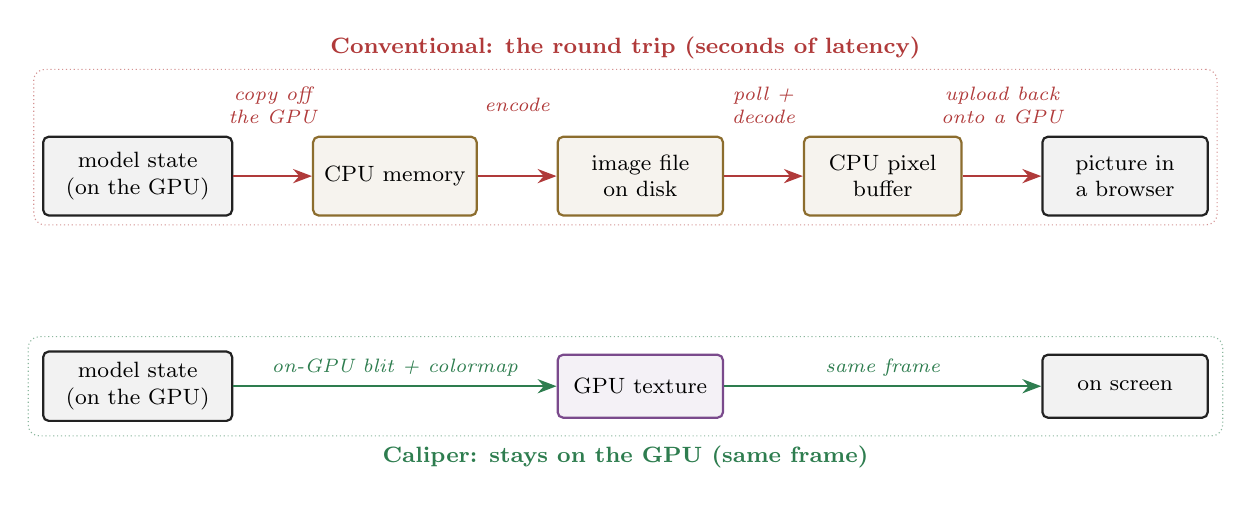
\begin{tikzpicture}[node distance=4mm and 6mm]
  % ---- conventional row ----
  \node[gpu, minimum width=24mm, minimum height=10mm] (a)
    {model state\\ (on the GPU)};
  \node[mem, right=10mm of a, minimum width=20mm, minimum height=10mm] (b)
    {CPU memory};
  \node[mem, right=10mm of b, minimum width=21mm, minimum height=10mm] (c)
    {image file\\ on disk};
  \node[mem, right=10mm of c, minimum width=20mm, minimum height=10mm] (d)
    {CPU pixel\\ buffer};
  \node[gpu, right=10mm of d, minimum width=21mm, minimum height=10mm] (e)
    {picture in\\ a browser};
  \draw[copyflow] (a) -- (b);
  \draw[copyflow] (b) -- (c);
  \draw[copyflow] (c) -- (d);
  \draw[copyflow] (d) -- (e);
  % step labels float ABOVE the box tops so they never collide with boxes
  \node[note, text=cCopy] (l1) at ($(a.east)!0.5!(b.west)+(0,9mm)$)
    {copy off\\ the GPU};
  \node[note, text=cCopy] (l2) at ($(b.east)!0.5!(c.west)+(0,9mm)$) {encode};
  \node[note, text=cCopy] (l3) at ($(c.east)!0.5!(d.west)+(0,9mm)$)
    {poll +\\ decode};
  \node[note, text=cCopy] (l4) at ($(d.east)!0.5!(e.west)+(0,9mm)$)
    {upload back\\ onto a GPU};
  % ---- caliper row ----
  \node[gpu, below=17mm of a, minimum width=24mm] (f)
    {model state\\ (on the GPU)};
  \node[host, minimum width=21mm] (g) at (f -| c) {GPU texture};
  \node[gpu, minimum width=21mm] (h) at (f -| e) {on screen};
  \draw[zeroflow] (f) -- node[above, note, text=cZero]
    {on-GPU blit + colormap} (g);
  \draw[zeroflow] (g) -- node[above, note, text=cZero] {same frame} (h);
  \begin{scope}[on background layer]
    \node[fit=(a)(e)(l1)(l2)(l3)(l4), draw=cCopy!55, densely dotted,
          rounded corners, inner sep=3pt,
          label={[cCopy,font=\footnotesize\bfseries]above:%
          Conventional: the round trip (seconds of latency)}] {};
    \node[fit=(f)(h), draw=cZero!55, densely dotted, rounded corners,
          inner sep=5pt, label={[cZero,font=\footnotesize\bfseries]below:%
          Caliper: stays on the GPU (same frame)}] {};
  \end{scope}
\end{tikzpicture}
\caption{The round trip every mainstream tool pays, against Caliper's
same-frame path.}
\label{fig:roundtrip}
\end{figure}

It is as if a security camera worked by printing each frame, mailing the
photograph, and scanning it at the other end. The picture arrives; the
\emph{event} is long over. In practice this means researchers sample sparsely
(every $N$ minutes, every epoch), and whole categories of fast dynamics ---
what happens in the first two hundred optimizer steps, how a representation
reorganizes during a loss spike --- are simply never seen by anyone.

The strange part: the data starts out on the same class of chip that draws
your screen. The round trip exists not because physics demands it, but
because the software worlds of \emph{computing} on a GPU and \emph{drawing}
with a GPU grew up separately and rarely share memory. That accident of
history is the entire problem Caliper solves.

\textbf{What ``solved'' looks like:} you click \emph{Train} and watch a
three-dimensional cloud of 2{,}000 handwritten digits --- positioned by the
network's own internal representation --- split from one gray blob into ten
colored lobes as the model learns to tell digits apart. Rotatable with a
mouse, updating live, on a laptop. No server. No browser. No files.

% ============================================================================
\section{Why nobody fixed this before}
% ============================================================================

\seclabelnote{Primary audience: technical readers; business readers get the
moat argument in \S5. This section is what separates an external paper from
internal docs --- it must establish that the problem is genuinely hard, not
merely neglected.}

Three walls stand between a training loop and a rendered pixel, and each one
independently forces the CPU round trip in existing tools:

\begin{enumerate}
  \item \textbf{The API wall.} Compute frameworks speak CUDA/MPS; renderers
        speak Vulkan/Metal/OpenGL. These APIs historically could not
        reference each other's memory. The escape hatches --- unified memory
        on Apple Silicon, \texttt{VK\_KHR\_external\_memory} + CUDA interop
        on NVIDIA --- are recent, fiddly, platform-specific, and rarely used
        outside game engines.
  \item \textbf{The process wall.} The standard tooling architecture puts
        visualization in a \emph{different process} (a web server) and often
        a different machine. Once you cross a process boundary, you are
        serializing; once you serialize GPU-resident data, the round trip is
        already lost.
  \item \textbf{The correctness wall.} Sharing memory between a training
        framework that is \emph{still writing} and a renderer that is
        \emph{reading} is a race by default. Getting it wrong doesn't crash
        politely; it renders yesterday's bytes or corrupts command streams.
        (We hit both --- \S7 documents the two races and the rules that
        survived them.)
\end{enumerate}

Each wall has a known workaround; the contribution is an architecture in
which all three are crossed \emph{at once}, portably, behind a contract small
enough to freeze. That is why the answer is a platform and not a patch to
TensorBoard.

% ============================================================================
\section{What it makes possible}
% ============================================================================

\seclabelnote{Primary audience: everyone --- this is the payoff section, and
it is deliberately placed before any mechanism. Screenshots/short clips go
here in the published version; each example below exists and runs today.}

The narrow reading of ``tensor visualization'' is heatmaps. The consequential
reading is: \textbf{the model's live internal state is in the same address
space as a renderer}, so an applet can compute \emph{any} transformation of
it --- on the GPU, mid-training --- and draw the result the same frame. The
tensor is the source; the visualization is derived
(Figure~\ref{fig:derive}):

\begin{figure}[ht]
\centering
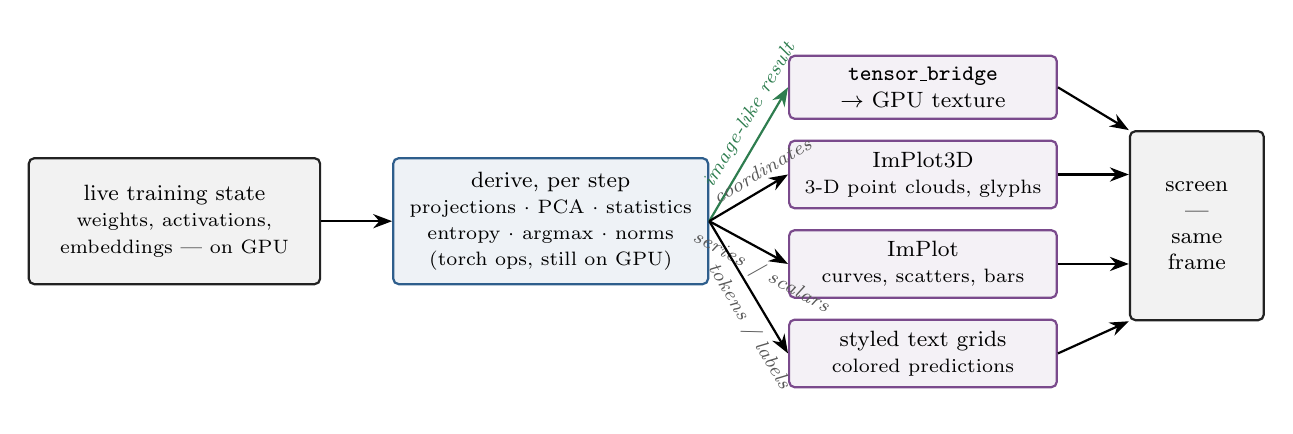
\begin{tikzpicture}[node distance=3mm and 10mm]
  \node[gpu, minimum width=37mm, minimum height=16mm] (t)
    {live training state\\ {\scriptsize weights, activations,}\\
     {\scriptsize embeddings --- on GPU}};
  \node[appl, right=9mm of t, minimum width=40mm, minimum height=16mm] (d)
    {derive, per step\\ {\scriptsize projections $\cdot$ PCA $\cdot$ statistics}\\
     {\scriptsize entropy $\cdot$ argmax $\cdot$ norms}\\
     {\scriptsize (torch ops, still on GPU)}};
  \node[host, right=10mm of d, minimum width=34mm, yshift=17mm] (tex)
    {\texttt{tensor\_bridge}\\ $\rightarrow$ GPU texture};
  \node[host, minimum width=34mm, below=2.5mm of tex] (p3)
    {ImPlot3D\\ {\scriptsize 3-D point clouds, glyphs}};
  \node[host, minimum width=34mm, below=2.5mm of p3] (p2)
    {ImPlot\\ {\scriptsize curves, scatters, bars}};
  \node[host, minimum width=34mm, below=2.5mm of p2] (txt)
    {styled text grids\\ {\scriptsize colored predictions}};
  \node[gpu, right=9mm of p3, minimum width=17mm, minimum height=24mm,
        yshift=-6.5mm] (s) {screen\\ ---\\ same\\ frame};
  \draw[flow] (t) -- (d);
  \draw[zeroflow] (d.east) -- node[pos=0.72, above, sloped, note, text=cZero]
    {image-like result} (tex.west);
  \draw[flow] (d.east) -- node[pos=0.78, above, sloped, note]
    {coordinates} (p3.west);
  \draw[flow] (d.east) -- node[pos=0.78, below, sloped, note]
    {series / scalars} (p2.west);
  \draw[flow] (d.east) -- node[pos=0.72, below, sloped, note]
    {tokens / labels} (txt.west);
  \draw[flow] (tex.east) -- (s.north west);
  \draw[flow] (p3.east) -- (s.west |- p3);
  \draw[flow] (p2.east) -- (s.west |- p2);
  \draw[flow] (txt.east) -- (s.south west);
\end{tikzpicture}
\caption{The tensor is the source; every visualization is a per-step
derivation over live state. Dense image-like results take the zero-copy
bridge; coordinate-style outputs flow through plotting libraries as small CPU
arrays, and the routes compose freely.}
\label{fig:derive}
\end{figure}

\begin{itemize}
  \item \textbf{EmbedScope --- geometry of learning.} A digit-classifier with
        a 3-neuron bottleneck; its activations \emph{are} 3-D coordinates.
        Two thousand test digits render as a live point cloud that visibly
        reorganizes from one blob into ten lobes as training runs. Hovering
        any point shows that digit's image and the model's current guess.
  \item \textbf{GPTScope --- a language model, transparent.} A small GPT
        trains live on Shakespeare. Attention heads render as sharpening
        heatmaps; sixteen heads reduce to two derived statistics and migrate
        across a scatter plot as they specialize; a logit lens renders ``when
        does the model decide?'' as a colored text grid; generated samples
        evolve from gibberish to iambic cadence over three minutes.
  \item \textbf{Geometry, live and zero-copy --- the completed ladder.} A
        network's \emph{output} can be a solid, not just an image: MeshScope
        draws a learned 2-D surface --- Lambert-lit, loss-colored, wireframe
        overlay --- straight from the GPU memory the optimizer writes, with zero
        copies of the geometry ever made; paint the target with the mouse and
        the net visibly chases the edit. On that base the ladder now runs to its
        top rungs. \textbf{TwinScope} drapes a live cotangent-Laplacian heat
        field (an MLP chasing a simulation) over a CAD heatsink housing at
        texture resolution --- state painted on a twin's shape
        (\texttt{geometry.v1\_2}, textures-on-meshes). \textbf{instance\_scope}
        renders one mesh times an imported \texttt{(N,16)} device pose tensor
        (optional per-instance tint) as $N$ objects on a 1--5{,}000 slider in a
        \emph{single} instanced draw --- ``1{,}000 objects, 1 draw call, 0 mesh
        copies'' (\texttt{geometry.v1\_3}, instanced populations). Every rung
        --- images $\rightarrow$ points $\rightarrow$ connected shapes
        $\rightarrow$ state-on-shapes $\rightarrow$ populations --- is
        byte-exact zero-copy on \emph{both} ecosystems (Metal/Apple Silicon and
        Vulkan/CUDA on an RTX~500 Ada; the v1\_2 rungs 2026-07-10, the v1\_3
        rungs 2026-07-11), behind one frozen additive C ABI.
  \item \textbf{Per-step surfaces.} Convolution kernels and projection
        matrices update ${\sim}8$ times per second --- every optimizer step,
        not every eval --- because the cost of showing a tensor no longer
        includes a trip through the CPU.
\end{itemize}

Two properties make these more than demos:

\begin{itemize}
  \item \textbf{Identical code, three backends.} The same applet binary
        renders via zero-copy Metal on a Mac, Vulkan/CUDA interop on a
        Windows/NVIDIA machine, and a CPU-staged OpenGL fallback anywhere
        else. The worst case is a working slow path, never a broken one.
  \item \textbf{Honest labeling.} The status line tells you which path ran
        (``GPU-resident --- zero CPU staging'' vs ``CPU-staged fallback'').
        The system never claims a fast path it didn't take.
\end{itemize}

% ============================================================================
\section{The business significance}
% ============================================================================

\seclabelnote{Primary audience: business. The argument is cost-of-blindness +
deleted infrastructure + portability = market coverage, with verification as
the de-risking close.}

\textbf{The cost of training blind.} GPU time is the dominant marginal cost
of model development, and the most expensive failure mode is the one
discovered late: a run that was doomed at step 500 but ran for twelve hours
because nobody could see inside it. Sparse, laggy observability is not an
inconvenience --- it is a multiplier on every failed run. Same-frame
visualization moves failure detection from \emph{post-mortem} to \emph{while
it is happening}, on the developer's own machine.

\textbf{Deleted infrastructure.} The incumbent architecture is a logging
library + a disk format + a server process + a browser stack. Caliper is one
native application; the visualization ``pipeline'' is a function call. For
teams, that is a support surface and a security surface that simply ceases to
exist; for laptops-and-workstations development (where an increasing share of
iteration happens, especially on Apple Silicon), it is the difference between
tooling you run and tooling you \emph{are running a service for}.

\textbf{Portability as market coverage.} The two hardware ecosystems that
matter --- Apple Silicon for local development, NVIDIA for serious training
--- have \emph{opposite} memory architectures (unified vs.\ discrete).
Caliper's contract never names a graphics API, which is why the NVIDIA
implementation landed without changing a single applet, and why the same
argument extends to future backends. A competitor must solve both memory
models \emph{and} reproduce the frozen-contract discipline to match the
portability claim.

\textbf{De-risked, not promised.} Every rendering path is verified
byte-for-byte against a CPU reference implementation by automated tests on
real hardware on both platforms. ``It works on both'' is a CI gate, not a
roadmap item.

\smallskip
\noindent{\small\itshape (Deliberately out of scope for v0.1 of this draft:
pricing/packaging, cloud story, team-scale collaboration. Flag for a later
revision once positioning is decided.)}

% ============================================================================
\section{The solution architecture}
% ============================================================================

\seclabelnote{Primary audience: research/engineering. From here down the
paper earns the claims made above. Tone shift is intentional and announced by
the structure.}

\subsection{One contract, three backends}

Applets --- the visualization programs --- never touch a graphics API. They
fill a plain C struct (\texttt{CaliperTensor}: data pointer, shape, strides,
dtype, and a \texttt{device} field saying where the bytes live) and hand it
to a frozen service ABI, \texttt{tensor\_bridge.v1}. Behind the host's
renderer seam, a backend turns it into a texture however that platform does
it best (Figure~\ref{fig:contract}):

\begin{figure}[ht]
\centering
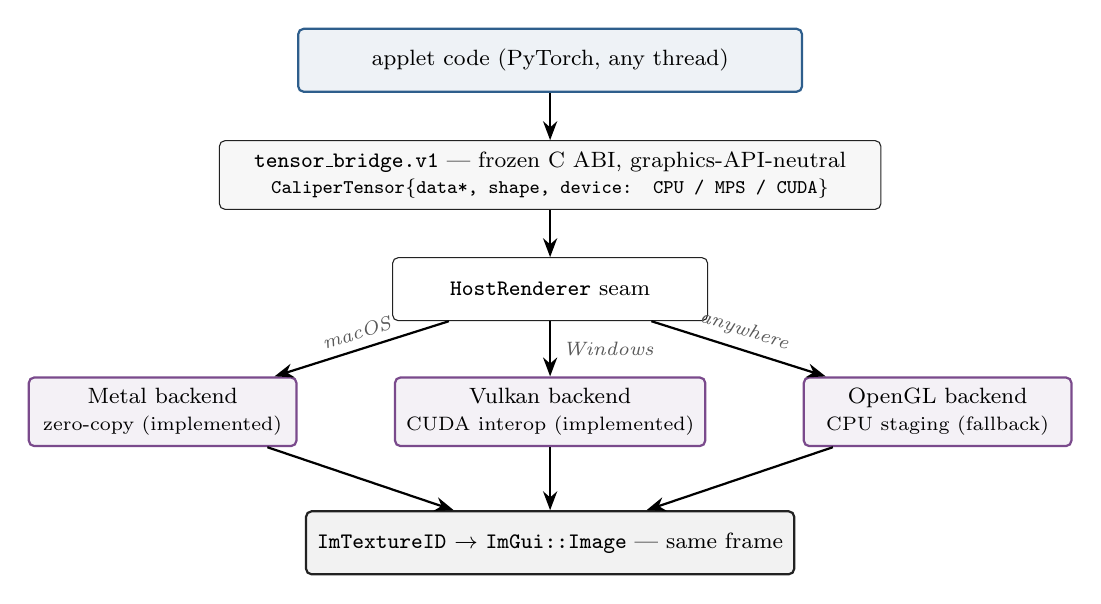
\begin{tikzpicture}[node distance=5mm and 5mm]
  \node[appl, minimum width=64mm] (app)
    {applet code (PyTorch, any thread)};
  \node[box, below=6mm of app, minimum width=84mm, fill=black!3] (bridge)
    {\texttt{tensor\_bridge.v1} --- frozen C ABI, graphics-API-neutral\\
     {\scriptsize \texttt{CaliperTensor\{data*, shape, device: CPU / MPS / CUDA\}}}};
  \node[box, below=6mm of bridge, minimum width=40mm] (seam)
    {\texttt{HostRenderer} seam};
  \node[host, below left=7mm and 12mm of seam, minimum width=34mm] (metal)
    {Metal backend\\ {\scriptsize zero-copy (implemented)}};
  \node[host, below=7mm of seam, minimum width=34mm] (vk)
    {Vulkan backend\\ {\scriptsize CUDA interop (implemented)}};
  \node[host, below right=7mm and 12mm of seam, minimum width=34mm] (gl)
    {OpenGL backend\\ {\scriptsize CPU staging (fallback)}};
  \node[gpu, below=24mm of seam, minimum width=52mm] (img)
    {\texttt{ImTextureID} $\rightarrow$ \texttt{ImGui::Image} --- same frame};
  \draw[flow] (app) -- (bridge);
  \draw[flow] (bridge) -- (seam);
  \draw[flow] (seam) -- node[above, sloped, note] {macOS} (metal);
  \draw[flow] (seam) -- node[right=1pt, note] {Windows} (vk);
  \draw[flow] (seam) -- node[above, sloped, note] {anywhere} (gl);
  \draw[flow] (metal) -- (img);
  \draw[flow] (vk) -- (img);
  \draw[flow] (gl) -- (img);
\end{tikzpicture}
\caption{One frozen contract; the renderer stays swappable forever. The
NVIDIA backend landed without changing a single applet.}
\label{fig:contract}
\end{figure}

\begin{table}[ht]
\centering\footnotesize
\begin{tabular}{@{}p{0.30\textwidth}p{0.40\textwidth}p{0.22\textwidth}@{}}
\toprule
Backend & Mechanism & Data crossings \\
\midrule
Metal / MPS (Apple Silicon) &
  unified memory: the tensor's storage \emph{is} an \texttt{MTLBuffer};
  handoff is a pointer cast + safety rules &
  0 host copies; 1 on-GPU blit \\
\addlinespace
Vulkan / CUDA (Win\-dows/NVIDIA), arbitrary tensor &
  Vulkan exports a VRAM buffer, CUDA imports it; one in-VRAM
  \texttt{cuMemcpyDtoD}; buffer$\rightarrow$image pass &
  0 host copies; 1 in-VRAM copy \\
\addlinespace
Vulkan / CUDA, \texttt{alloc\_shared} &
  the tensor's backing store \emph{is} the interop buffer; kernels write
  texture memory in place &
  0 host copies; \textbf{0 in-VRAM copies} \\
\addlinespace
Vulkan / CUDA, exportable-pool tensor (bridge v1.2, \S6.5) &
  the applet's pool block is imported into Vulkan once; the pass reads the
  tensor at its byte offset, in place &
  0 host copies; \textbf{0 in-VRAM copies} \\
\addlinespace
OpenGL / CPU (anywhere) &
  CPU colormap + one texture upload &
  1 host staging + 1 upload \\
\bottomrule
\end{tabular}
\caption{The data-crossing ladder, best to worst. Every row is implemented;
the native rows are pixel-exact-verified on real hardware.}
\label{tab:ladder}
\end{table}

The returned texture id casts directly to an \texttt{ImTextureID}, and the
applet draws it with \texttt{ImGui::Image} in the same frame.

\textbf{Definition discipline.} ``Zero-copy'' in this paper means: the
tensor's \emph{data} never leaves the GPU and never transits host memory. One
GPU-side buffer$\rightarrow$texture pass remains (samplers read textures, not
raw buffers); it runs at memory bandwidth, on-device. For an \emph{arbitrary}
framework-allocated CUDA tensor, one in-VRAM copy is the floor (the
framework's caching allocator does not produce exportable allocations); the
literal zero-copy rungs are \texttt{alloc\_shared}, where training kernels
write the texture's own backing memory, and the exportable pool (\S6.5),
where the tensor is \emph{born} in memory the renderer can import. The paper
--- like the product's status lines --- reserves each label for the path that
earns it.

\subsection{Apple Silicon: aliasing under unified memory}

CPU and GPU share one pool of physical RAM, so a PyTorch MPS tensor's storage
already is the object Metal renders from. What makes the cast \emph{safe}
rather than merely possible: the frozen struct has no storage-offset channel,
so the adapter \textbf{rejects} non-contiguous tensors and views with nonzero
storage offsets rather than silently copying or --- worse --- silently
addressing the wrong texels. Repairs (\texttt{.contiguous()},
\texttt{.clone()}) happen in applet code, where their cost is visible. A GPU
compute pass applies colormaps for float heatmaps; a blit path handles direct
RGBA. Figure~\ref{fig:metalseq} shows the handoff.

\begin{figure}[ht]
\centering
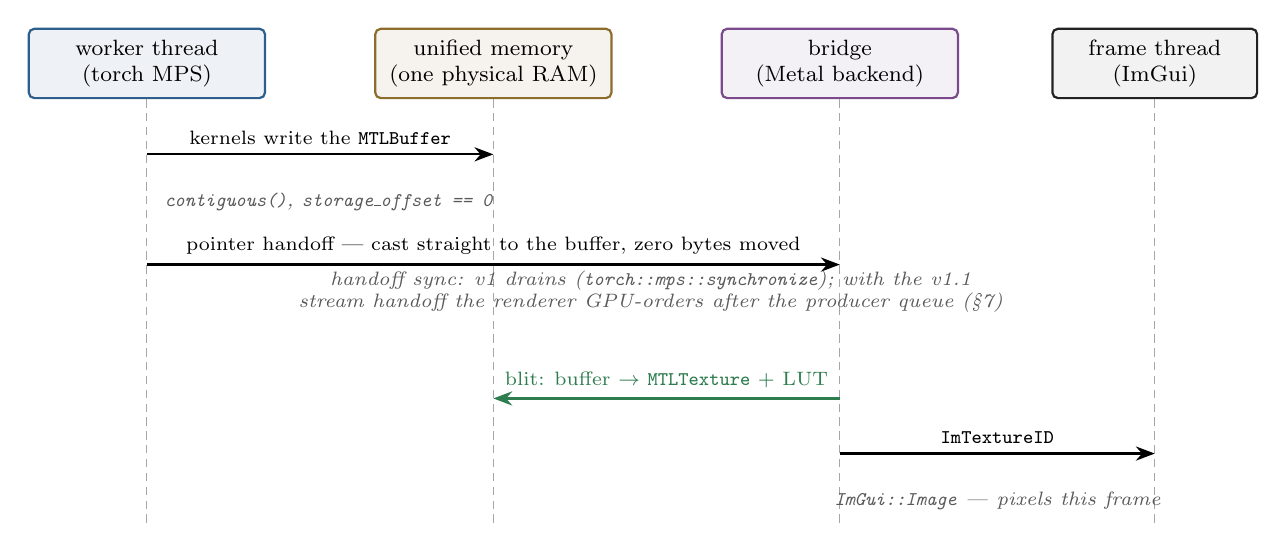
\begin{tikzpicture}[x=1mm, y=1mm]
  % lifeline heads
  \node[appl, minimum width=30mm] (W) at (0,0)   {worker thread\\ (torch MPS)};
  \node[mem,  minimum width=30mm] (U) at (44,0)  {unified memory\\ (one physical RAM)};
  \node[host, minimum width=30mm] (B) at (88,0)  {bridge\\ (Metal backend)};
  \node[gpu,  minimum width=26mm] (F) at (128,0) {frame thread\\ (ImGui)};
  % lifelines
  \foreach \n in {W,U,B,F} \draw[life] (\n.south) -- ($(\n.south)+(0,-54)$);
  % messages
  \draw[msg] ($(W.south)+(0,-7)$)  -- node[above]
    {kernels write the \texttt{MTLBuffer}} ($(U.south)+(0,-7)$);
  \node[note, anchor=west] at ($(W.south)+(1,-13)$)
    {\texttt{contiguous()}, \texttt{storage\_offset == 0}};
  \draw[msg] ($(W.south)+(0,-21)$) -- node[above]
    {pointer handoff --- cast straight to the buffer, zero bytes moved}
    ($(B.south)+(0,-21)$);
  \node[note] at (64,-29)
    {handoff sync: v1 drains (\texttt{torch::mps::synchronize}); with the
     v1.1\\ stream handoff the renderer GPU-orders after the producer
     queue (\S7)};
  \draw[msg, zeroflow] ($(B.south)+(0,-38)$) -- node[above]
    {blit: buffer $\rightarrow$ \texttt{MTLTexture} + LUT}
    ($(U.south)+(0,-38)$);
  \draw[msg] ($(B.south)+(0,-45)$) -- node[above]
    {\texttt{ImTextureID}} ($(F.south)+(0,-45)$);
  \node[note, anchor=east] at ($(F.south)+(2,-51)$)
    {\texttt{ImGui::Image} --- pixels this frame};
\end{tikzpicture}
\caption{The Apple Silicon handoff: the tensor and the texture source are the
same physical memory; safety comes from rejection rules and the negotiated
sync ladder, not from copies.}
\label{fig:metalseq}
\end{figure}

\subsection{Windows/NVIDIA: external-memory interop}

Discrete GPUs separate VRAM from system RAM, so zero-copy means \emph{keep it
in VRAM and make the two APIs share the allocation}. The direction is the
non-obvious part: the \textbf{renderer exports} (Vulkan external memory,
opaque Win32 handle) and \textbf{CUDA imports} --- because the training
framework's allocator can't export. Device pairing is UUID-driven (the Vulkan
device and CUDA device must be the same physical silicon; a hybrid-GPU
mismatch disables interop rather than corrupting). Colormapping runs as a
SPIR-V compute pass byte-identical to the CPU reference. The host loads the
CUDA \emph{driver} API at runtime from the system's own driver --- no CUDA
toolkit dependency; machines without NVIDIA hardware build and run unchanged.
Figure~\ref{fig:vkseq} shows the flow.

\begin{figure}[ht]
\centering
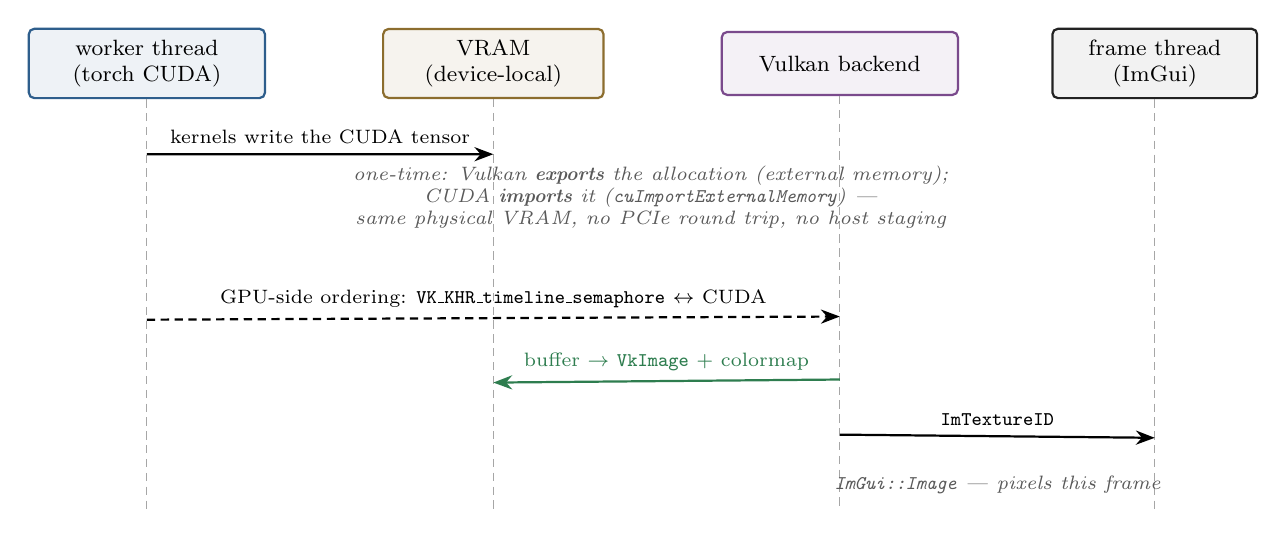
\begin{tikzpicture}[x=1mm, y=1mm]
  \node[appl, minimum width=30mm] (T) at (0,0)   {worker thread\\ (torch CUDA)};
  \node[mem,  minimum width=28mm] (V) at (44,0)  {VRAM\\ (device-local)};
  \node[host, minimum width=30mm] (R) at (88,0)  {Vulkan backend};
  \node[gpu,  minimum width=26mm] (F) at (128,0) {frame thread\\ (ImGui)};
  \foreach \n in {T,V,R,F} \draw[life] (\n.south) -- ($(\n.south)+(0,-52)$);
  \draw[msg] ($(T.south)+(0,-7)$) -- node[above]
    {kernels write the CUDA tensor} ($(V.south)+(0,-7)$);
  \node[note] at (64,-17)
    {one-time: Vulkan \textbf{exports} the allocation (external memory);\\
     CUDA \textbf{imports} it (\texttt{cuImportExternalMemory}) ---\\
     same physical VRAM, no PCIe round trip, no host staging};
  \draw[msg, densely dashed] ($(T.south)+(0,-28)$) -- node[above]
    {GPU-side ordering: \texttt{VK\_KHR\_timeline\_semaphore}
     $\leftrightarrow$ CUDA} ($(R.south)+(0,-28)$);
  \draw[msg, zeroflow] ($(R.south)+(0,-36)$) -- node[above]
    {buffer $\rightarrow$ \texttt{VkImage} + colormap}
    ($(V.south)+(0,-36)$);
  \draw[msg] ($(R.south)+(0,-43)$) -- node[above]
    {\texttt{ImTextureID}} ($(F.south)+(0,-43)$);
  \node[note, anchor=east] at ($(F.south)+(2,-49)$)
    {\texttt{ImGui::Image} --- pixels this frame};
\end{tikzpicture}
\caption{The Windows/NVIDIA path: one VRAM allocation shared across APIs,
ordered by GPU-side semaphores; no CPU thread waits on the hot path.}
\label{fig:vkseq}
\end{figure}

\subsection{The degradation ladder}

Every acceptance failure --- foreign device, non-contiguous layout, absent
interop, exotic allocator --- returns \texttt{false} and takes the next rung
down, ending at the CPU-staged path. A failed fast path is a staged frame,
never a crash and never a wrong image. This is why the same applet is
demoable on a MacBook, a gaming PC, and a VM.

\subsection{Removing the arbitrary-tensor floor: the exportable pool
(bridge v1.2)}
\label{sec:pool}

Table~\ref{tab:ladder}'s ``arbitrary tensor'' row carries one in-VRAM copy
per update because exportability is an \emph{allocation-time} property:
memory obtained from the framework's default allocator cannot be retrofitted
with a shareable handle. Bridge v1.2 therefore moves the fix to allocation
time. The SDK's \texttt{ExportablePool} is a torch memory pool whose blocks
are created with \texttt{cuMemCreate} and a shareable OS handle; an applet
materializes exactly the tensors it wants to display inside the pool's scope,
and everything else in the process keeps the default allocator. The host
imports each block into Vulkan \emph{once} (\texttt{import\_allocation}) and
thereafter updates textures \emph{directly from the block at the tensor's
byte offset} (\texttt{update\_texture\_from\_alloc}) --- the per-update
in-VRAM copy no longer exists (Figure~\ref{fig:pool}).

\begin{figure}[ht]
\centering
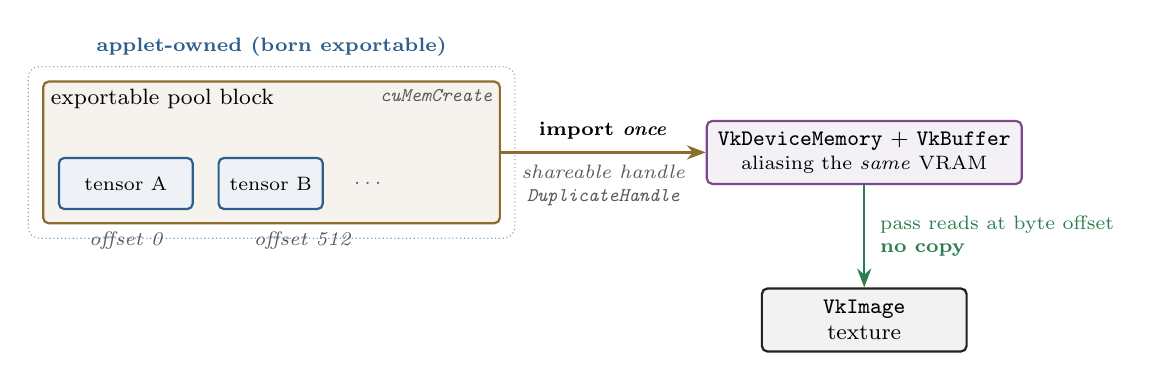
\begin{tikzpicture}[node distance=7mm and 12mm]
  \node[mem, minimum width=58mm, minimum height=18mm] (blk) {};
  \node[font=\footnotesize, anchor=north west, inner sep=3pt] at (blk.north west)
    {exportable pool block};
  \node[note, anchor=north east, inner sep=3pt] at (blk.north east)
    {\texttt{cuMemCreate}};
  \node[appl, minimum width=17mm, minimum height=6.5mm, anchor=south west,
        font=\scriptsize] at ($(blk.south west)+(2mm,1.8mm)$) (t0) {tensor A};
  \node[appl, minimum width=13mm, minimum height=6.5mm, right=3mm of t0,
        font=\scriptsize] (t1) {tensor B};
  \node[note, right=2.5mm of t1] {\dots};
  \node[note, anchor=north] at ($(t0.south)+(0,-1.5mm)$) {offset 0};
  \node[note, anchor=north] at ($(t1.south)+(4mm,-1.5mm)$) {offset 512};
  \node[host, right=26mm of blk, minimum width=38mm] (vkmem)
    {\texttt{VkDeviceMemory} + \texttt{VkBuffer}\\[-1pt]
     {\scriptsize aliasing the \emph{same} VRAM}};
  \node[gpu, below=13mm of vkmem, minimum width=26mm] (tex)
    {\texttt{VkImage}\\ texture};
  \draw[flow, draw=cMem] (blk) -- node[above=1pt, font=\scriptsize\bfseries]
    {import \emph{once}} node[below=1pt, note]
    {shareable handle\\ \texttt{DuplicateHandle}} (vkmem);
  \draw[zeroflow] (vkmem) -- node[right=2pt, font=\scriptsize, align=left]
    {pass reads at byte offset\\ \textbf{no copy}} (tex);
  \begin{scope}[on background layer]
    \node[fit=(blk)(t0)(t1), draw=cAppl!60, densely dotted, rounded corners,
          inner sep=5pt,
          label={[cAppl,font=\scriptsize\bfseries]above:applet-owned (born exportable)}] {};
  \end{scope}
\end{tikzpicture}
\caption{Bridge v1.2: tensors born in the exportable pool update textures
with zero copies of their data. Blocks are 2\,MiB-granularity allocations;
torch sub-allocates tensors at 512-byte alignment, which satisfies the
renderer's offset-alignment gate.}
\label{fig:pool}
\end{figure}

The revision is additive (the v1/v1.1 tables are untouched; hosts advertise a
capability bit) and fails closed at every gate: a declined import, a
misaligned offset, an out-of-bounds window, or a released allocation each
return \texttt{false} and the applet falls back to the copying path --- never
a crash, never a wrong image. The floor of Table~\ref{tab:ladder} is thus
\emph{per allocation origin}: it persists only for memory born unshareable.
The path is hardware-verified: byte-exact readback at multiple offsets
through the imported block, and a live training applet whose status line
reports \emph{``zero-copy (imported pool)''} only while the imported path is
actually the one on screen. (A companion technical report,
\texttt{docs/report/zerocopy-import-v12}, documents the design and its
verification in full.)

% ============================================================================
\section{Synchronization: the part that bites}
% ============================================================================

\seclabelnote{Primary audience: research/engineering. This section carries
the paper's credibility with systems readers --- it is where most naive
implementations die, and we present it races-first.}

Sharing memory between a producer that is still writing and a consumer that
renders is only correct if \emph{when} is as disciplined as \emph{where}.
Caliper's answer is a two-rung negotiated ladder:

\begin{itemize}
  \item \textbf{v1 --- drain.} Synchronize the producer device fully before
        handoff (sync-then-update). Always correct; costs one full-device
        barrier, paid once at the handoff, never per frame.
  \item \textbf{v1.1 --- stream-ordered handoff.} The adapter publishes the
        producer's queue/stream in the tensor struct; the renderer GPU-orders
        its work after the producer's (per-texture \texttt{MTLSharedEvent} on
        Metal; a shared timeline semaphore riding the producer's CUDA stream
        on Vulkan). No CPU thread waits on the hot path. Hosts advertise the
        capability; adapters degrade to the drain automatically.
\end{itemize}

Two hard-won findings, offered as cautionary results:

\begin{enumerate}
  \item \textbf{PyTorch's public MPS stream calls are not internally
        serialized} (we established this by disassembly after crashes in
        three different costumes). Handing off while the training thread
        encodes corrupts command-buffer state. All MPS-touching handoff work
        must run as one block on the framework's own stream dispatch queue.
  \item \textbf{CUDA's thread-safety is contractual --- we pinned it
        anyway.} The MPS lesson was precisely that ``should be safe'' is not
        evidence; a 500-handoff concurrent-training stress test holds the
        property empirically.
\end{enumerate}

And one honest measurement: eliding the drain did \textbf{not} improve
training throughput ($\approx 0$ delta on the benchmark machine --- the
training loop's own per-step \texttt{loss.item()} sync dominates). The
verified win is ordering correctness plus removal of frame-thread stalls.
Papers in this genre routinely imply throughput wins they haven't measured;
we measured, and report what we found.

% ============================================================================
\section{Verification: pixel-exact or it didn't happen}
% ============================================================================

\seclabelnote{All audiences, one page. For business readers this is the
de-risking section; for researchers it is the methods section.}

The claim ``the GPU path is equivalent to the reference'' is a \emph{byte}
claim, tested as one. A single CPU function is the source of truth for
colormapping; every GPU implementation (Metal compute, Metal blit, SPIR-V
compute, Vulkan copy) must read back \textbf{byte-identical} output across
adversarial sizes (non-multiple-of-16, ragged shapes), NaN inputs, and
degenerate ranges --- in an automated windowed test harness, per backend,
every CI run, including on real NVIDIA hardware. The stream-ordered path adds
a burst test: eight overlapping updates ordered only by semaphores must land
byte-exact. The imported-allocation path (\S\ref{sec:pool}) adds rows that
must read back byte-exact \emph{at nonzero byte offsets} through an imported
block. Reading device buffers back for these comparisons is itself
platform-shaped: torch MPS tensors import as \emph{private-storage} Metal
buffers whose bytes the host cannot read directly, so the gate stages them
through a blit --- the same shape the discrete-VRAM Vulkan path already
required. Failure modes are designed to be loud: acceptance violations log and
reject rather than render a plausible-but-wrong image.

% ============================================================================
\section{Limits and non-claims}
% ============================================================================

\seclabelnote{Research audience explicitly; business audience implicitly ---
a paper that states its limits is a paper whose claims can be trusted.}

\begin{itemize}
  \item Arbitrary framework-allocated CUDA tensors carry a one in-VRAM-copy
        floor \textbf{unless allocated from Caliper's exportable pool, which
        removes it}; the floor persists only for memory born unshareable.
  \item The v1 contract requires contiguous, offset-0 tensors; views are
        rejected, not repaired.
  \item Dense outputs (heatmaps, feature maps, attention grids) and the full
        geometry ladder (point clouds, lines, indexed meshes,
        textures-on-meshes, instanced populations --- \texttt{geometry.v1}
        through \texttt{v1\_3}, R0--R3) all ride zero-copy paths, byte-exact on
        both ecosystems; only small derived series (curves, scatters, glyph
        clouds) still flow through plotting libraries as CPU arrays ---
        kilobytes, and the routes compose freely.
  \item The OpenGL fallback stages through the CPU by design; it exists so
        the worst case is slow, not broken.
  \item Same-frame visualization does not by itself accelerate training; its
        value is observational (\S7's measurement note).
  \item Single-machine, in-process by design. Remote/cluster training is a
        different problem (and largely re-introduces the round trip that
        distributed tooling rightly accepts); this paper claims the local
        loop.
\end{itemize}

% ============================================================================
\section{Implications and outlook}
% ============================================================================

For the \textbf{general reader}: instruments change what gets studied. When
the microscope got a video feed, biology got cell dynamics as a field.

For \textbf{business}: the local development loop is where iteration speed
compounds; tooling that deletes seconds from every look-inside changes how
often people look.

For \textbf{research}: most interpretability is post-hoc --- artifacts of
finished training. Per-step, in-the-loop observation makes \emph{training
dynamics} (representation reorganization, head specialization timing,
loss-spike anatomy) a first-class observable. The platform's applet model
means a new visualization is a new derivation over live state --- a torch op
and a draw call --- not a new pipeline.

On the platform's own trajectory: the core that does all of this --- the applet
contract, the host-neutral services, and the zero-copy renderer with its
completed geometry ladder --- is now extractable as an embeddable library
(\texttt{libcaliper}) behind a small C ABI, so a second host can vend the same
applets without owning the machinery. A GLFW-free native host already runs the
applets zero-copy on Apple Silicon (Metal/MPS); the Windows/NVIDIA embedding
path is written but its hardware verification is pending the next Windows
session, and a full sibling host remains a design-gated future, not a claim.

% ============================================================================
\appendix
\section{The bridge contract (abridged)}
% ============================================================================

The load-bearing property is what the contract does \emph{not} contain: no
graphics-API type appears anywhere. Textures cross the ABI as an opaque
64-bit id; the host keeps an id~$\rightarrow$~backend-handle table, so the
renderer behind the seam is swappable without touching an applet. The struct
below is frozen (immutable once published); later revisions (v1.1's
capability query and stream field, v1.2's imported allocations,
\S\ref{sec:pool}) are additive --- prefix-identical structs and new
capability bits, so old applets run on new hosts and vice versa.

\begin{lstlisting}
typedef uint64_t CaliperTextureId;   /* opaque; 0 = invalid; castable to
                                        ImTextureID for ImGui::Image */

typedef struct CaliperTensorBridgeV1 {
    uint32_t struct_size;

    /* Mirror a 3-D (H,W,C<=4) u8 tensor as a texture. GPU-resident on the
       native backends; CPU-staged on the GL fallback. 0 on failure. */
    CaliperTextureId (*texture_from_tensor)(const CaliperTensor* t,
                                            uint32_t flags);

    /* Re-upload into an existing texture (same shape/dtype). */
    bool (*update_texture)(CaliperTextureId tex, const CaliperTensor* t);
    void (*release_texture)(CaliperTextureId tex);

    /* Colormap a 2-D (H,W) f32 tensor through a built-in LUT, scaling
       [vmin,vmax] -> [0,1]. Identical numeric output on every backend. */
    CaliperTextureId (*texture_from_tensor_mapped)(const CaliperTensor* t,
                                                   int32_t colormap,
                                                   float vmin, float vmax,
                                                   uint32_t flags);

    /* Literal zero-copy: allocate tensor memory that IS the texture's
       backing store; the applet's kernels write it in place. */
    bool (*alloc_shared)(CaliperDType dtype, int32_t ndim,
                         const int64_t* shape,
                         CaliperTensor* out_tensor,
                         CaliperTextureId* out_texture);
    void (*free_shared)(CaliperTextureId tex);
} CaliperTensorBridgeV1;
\end{lstlisting}

\noindent
Acceptance rules (violations return 0/\texttt{false} and log --- never a
misinterpreted texture): 2-D f32 for the mapped path; 3-D u8 for the direct
path; contiguous row-major layout; the tensor's device must be the CPU or the
active backend's device. The v1.2 additions extend the same table with the
imported-block path of \S\ref{sec:pool},
\begin{center}\footnotesize
\texttt{import\_allocation} \quad \texttt{release\_allocation} \quad
\texttt{update\_texture\_from\_alloc}
\end{center}
\noindent
behind the \texttt{CALIPER\_BRIDGE\_CAP\_IMPORT\_ALLOC} capability bit.

% ============================================================================
\section{Verification matrix}
% ============================================================================

Every row below shipped and is green as of July 2026. ``Byte-exact'' means
\texttt{==} on the RGBA8 readback against the single CPU reference function,
no tolerances.

\begin{center}\footnotesize
\begin{tabular}{@{}p{0.34\textwidth}p{0.30\textwidth}p{0.16\textwidth}l@{}}
\toprule
Path & Test & Hardware & Status \\
\midrule
Metal compute (f32 colormap) & \S16 matrix: 3 colormaps, ragged sizes,
  NaN, degenerate ranges; byte-exact & Apple M-series & green \\
Metal blit (u8 RGBA) & direct-upload matrix; byte-exact & Apple M-series &
  green \\
Metal stream-ordered handoff & per-texture \texttt{MTLSharedEvent}
  ordering; concurrent-training stress & Apple M-series & green \\
\addlinespace
Vulkan CPU-staged (portable) & the same \S16 matrix on the Vulkan backend
  & any ICD (CI: lavapipe) & green \\
Vulkan/CUDA interop (arbitrary tensor) & device tensor
  $\rightarrow$ \texttt{"compute"} path; byte-exact at 4$\times$4,
  5$\times$3, 17$\times$9 & RTX 500 Ada & green \\
Vulkan/CUDA \texttt{alloc\_shared} & in-place device write reads back
  pixel-exact; no copy & RTX 500 Ada & green \\
Vulkan/CUDA pipelined sync & 8-update burst ordered only by timeline
  semaphores; byte-exact final frame & RTX 500 Ada & green \\
\addlinespace
Imported allocation, f32 (\S\ref{sec:pool}) & byte-exact at offsets 0 and
  512 through \texttt{"compute-imported"} & RTX 500 Ada & green \\
Imported allocation, u8 & \texttt{"blit-imported"} at offset 512;
  byte-exact & RTX 500 Ada & green \\
Imported allocation, negative rows & misaligned offset, out-of-bounds
  window, released id: \texttt{false}, pixels untouched & RTX 500 Ada &
  green \\
Imported allocation, lifecycle & 50$\times$ import/release, ids strictly
  increasing; live-app cancel/relaunch & RTX 500 Ada & green \\
\addlinespace
OpenGL fallback & the \S16 matrix, CPU-staged; live-app fallback run &
  any & green \\
\bottomrule
\end{tabular}
\captionof{table}{Path $\times$ test $\times$ hardware, distilled from the
internal test documentation (unit + gfx + torch suites; the gfx suite alone
is 22 cases / 1030 assertions as of this draft).}
\end{center}

% ============================================================================
\section{Glossary for the general reader}
% ============================================================================

\begin{description}\small
  \item[Tensor] a multi-dimensional array of numbers --- the universal
        container for everything inside a neural network.
  \item[GPU / VRAM] the processor that draws your screen and (in ML) does the
        training math; VRAM is its private, very fast memory.
  \item[Unified memory] Apple Silicon's design where CPU and GPU share one
        pool of physical RAM, so ``moving'' data between them can be free.
  \item[Texture] the GPU-native image format the renderer samples from when
        putting pixels on screen.
  \item[Frame] one full refresh of the screen (typically 1/60th of a
        second); ``same frame'' means computed and displayed with no refresh
        in between.
  \item[Interop] two APIs agreeing to reference the same memory instead of
        copying between their private worlds.
  \item[Semaphore] a GPU-side signal used to order work (``draw only after
        the training kernel finished writing'') without making a CPU thread
        wait.
\end{description}

\end{document}
